\chapter{Conclusão}

Após todas as iterações de análise das métricas previstas a serem coletadas, pode-se agora, responder o indicador final, o qual era previsto ao final de tudo.

Portanto, ao ter uma média final das métricas previstas, pode-se agora analisar e responder as perguntas previstas no GQM, que são as seguintes:

\section{Engrena}

\begin{itemize}
\item Q1.1 - Qual a satisfação do cliente em relação a participação dele no processo?

BOM

\item Q1.2 - Qual a satisfação do cliente com o produto?

NÃO SE APLICA

\item Q1.3 - Qual o entendimento do cliente em relação ao processo?

BOM

\item Q2.1 - Quantas atividades do modelo de maturidade aderiram ao processo?

12 ATIVIDADES

\item Q2.2 - Quantas atividades do modelo de maturidade foram estudadas?

NÃO SE APLICA

\item Q3.1 - Qual o tamanho do processo atual?

17 ATIVIDADES

\item Q3.2 - Qual o esforço da equipe em horas?

EM MÉDIA 3 HORAS POR ATIVIDADE

\item Q3.3 - Qual a produtividade da equipe?

NÃO SE APLICA

\item Q3.4 - Qual o tempo gasto para realização de cada atividade?


\begin{figure}[H]
  \center
  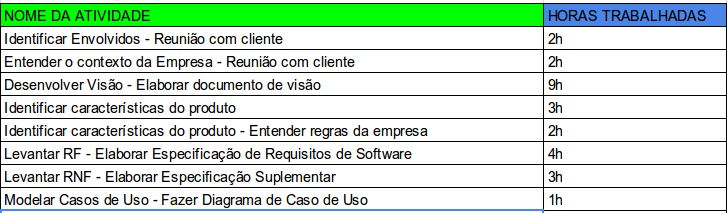
\includegraphics[width=0.7\textwidth]{figuras/tempo-atv1}
  \caption{Horas por Atividade}
  \label{fig:tempo-atv1}
\end{figure}

\item Q4.1 - Quanto custa o processo?

R\$ 1591,20

\item Q4.2 - Quanto custa cada atividade do processo?


\begin{figure}[H]
  \center
  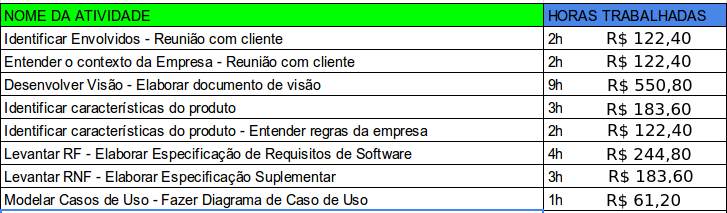
\includegraphics[width=0.7\textwidth]{figuras/custo-atv1}
  \caption{Custo por Atividade}
  \label{fig:custo-atv1}
\end{figure}

\item Q4.3 - Quanto custará a aderência de uma atividade do modelo de maturidade?

Em Média R\$ 100,00


\end{itemize}

\section{Eletrojun}

\begin{itemize}
\item Q1.1 - Qual a satisfação do cliente em relação a participação dele no processo?

MÉDIO

\item Q1.2 - Qual a satisfação do cliente com o produto?

NÃO SE APLICA

\item Q1.3 - Qual o entendimento do cliente em relação ao processo?

MÉDIO

\item Q2.1 - Quantas atividades do modelo de maturidade aderiram ao processo?

09 ATIVIDADES

\item Q2.2 - Quantas atividades do modelo de maturidade foram estudadas?

NÃO SE APLICA

\item Q3.1 - Qual o tamanho do processo atual?

20 ATIVIDADES

\item Q3.2 - Qual o esforço da equipe em horas?

EM MÉDIA 1,5 HORAS POR ATIVIDADE

\item Q3.3 - Qual a produtividade da equipe?

NÃO SE APLICA

\item Q3.4 - Qual o tempo gasto para realização de cada atividade?


\begin{figure}[H]
  \center
  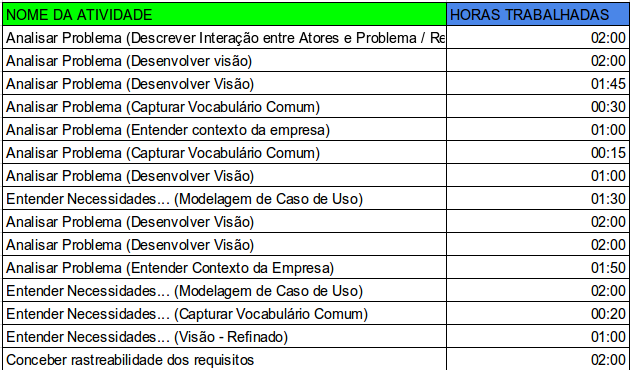
\includegraphics[width=0.7\textwidth]{figuras/tempo-atv2}
  \caption{Horas por Atividade}
  \label{fig:tempo-atv2}
\end{figure}

\item Q4.1 - Quanto custa o processo?

R\$ 1053,40

\item Q4.2 - Quanto custa cada atividade do processo?


\begin{figure}[H]
  \center
  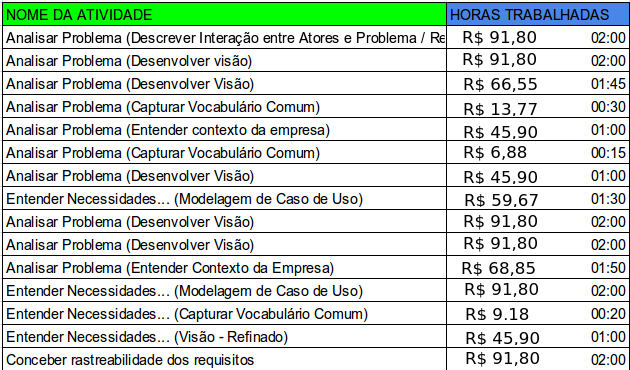
\includegraphics[width=0.7\textwidth]{figuras/custo-atv2}
  \caption{Custo por Atividade}
  \label{fig:custo-atv2}
\end{figure}

\item Q4.3 - Quanto custará a aderência de uma atividade do modelo de maturidade?

EM MÉDIA R\$ 100,00

\end{itemize}
